\section{Trajectory Optimization}
\label{sec:trajectory_optimization}

A trajectory optimization is a set of mathematical techniques, which is used to find an ideal or the best behavior for a dynamic system, or also known as optimal trajectory. In order to describe mathematically what is understood as the "best" trajectory, an \emph{objective function} should be defined \cite{kelly2017introduction}. Moreover, the optimization solver adjust a set of \emph{decision variables} in order to minimize the objective function.\\
In the present section, it is described the process to identify the optimal values of the decision variables, with the objective of fitting the dynamics of the thermal system into a model which is considered to be correct. 

\subsection{Objective function}
As a first step, the temperature $T_z$, obtained with a finite difference approximation of the Equation \ref{eq:energy_balance}, it is considered to be the ground truth of the room temperature, assuming that the values of $C_z$, $R_w$ and $gA$ presented in Table \ref{tab:constants} are correct. The discretization processes is developed in the next equation

\begin{equation}
T_{z,i+1} = \Delta t \cdot \left( \frac{\dot{Q}_{h,i} + gA \cdot \dot{Q}_{sun, i} + \dot{Q}_{g,i}}{C_z} + \frac{T_{z,i}-T_{a,i}}{R_w \cdot C_z} \right) + T_{z,i}
\label{eq:finite_difference_real}
\end{equation}
The value $\Delta t = 3600s$ was selected based on the sampling time of historical data.\\

Subsequently, a model $\tilde{T_z}$ is generated as it is shown in Equation \ref{eq:finite_difference_model}. This model is dependent on the variable vector $\mathbf{p} = \begin{bmatrix}
\tilde{C_z} & \tilde{R_w} & \tilde{gA} \end{bmatrix}^\top$, which its numerical value will be updated by the optimization solver. For that, an initial value of each is proposed to be relatively close to the ground truth, with the intention of making the algorithm to converge faster and avoiding it to get stuck in local minima. The numerical values used as initial guess are shown in Table \ref{tab:initial_guess}

\begin{equation}
\tilde{T}_{z,i+1} = \Delta t \cdot \left( \frac{\dot{Q}_{h,i} + \tilde{gA} \cdot \dot{Q}_{sun, i} + \dot{Q}_{g,i}}{\tilde{C}_z} + \frac{\tilde{T}_{z,i}-T_{a,i}}{\tilde{R}_w \cdot \tilde{C}_z} \right) + \tilde{T}_{z,i}
\label{eq:finite_difference_model}
\end{equation}


\begin{table}[H]
\centering
\begin{tabular}{c|c}
Variable & Value\\
\hline
\hline
$\tilde{C}_z$ & 1000000 J/K\\
$\tilde{R}_w$ & 1 K/W\\
$\tilde{gA}$ & $0.1\cdot1$ m$^2$ 
\end{tabular}
\caption{Initial guess of the decision variables.}
\label{tab:initial_guess}
\end{table}

As a next step, the objective function, or also known as \emph{cost function} is defined, it will determine how well the model $\tilde{T}_{z}$ is performing, using as a reference the ground truth model $T_{z}$. The Mean Squared Error (MSE) is perhaps the simplest and most common cost function, and the optimizer will try to minimize its value. To calculate it, the difference between the correct value $T_{z}$ and the model $\tilde{T}_{z}$ is taken for each sample, and averaging it across the whole set of samples $N$. The mathematical definition of this trajectory optimization problem is presented in Equation \ref{Eq:Cost_function}
\begin{equation}
\underset{\mathbf{p}}{\text{minimize}}\,\,\,\frac{1}{N}\sum_{i=1}^{N} (T_{z,i}-\tilde{T}_{z,i}(\mathbf{p}))^2 
\label{Eq:Cost_function}
\end{equation}

\begin{figure}[H]
\centering
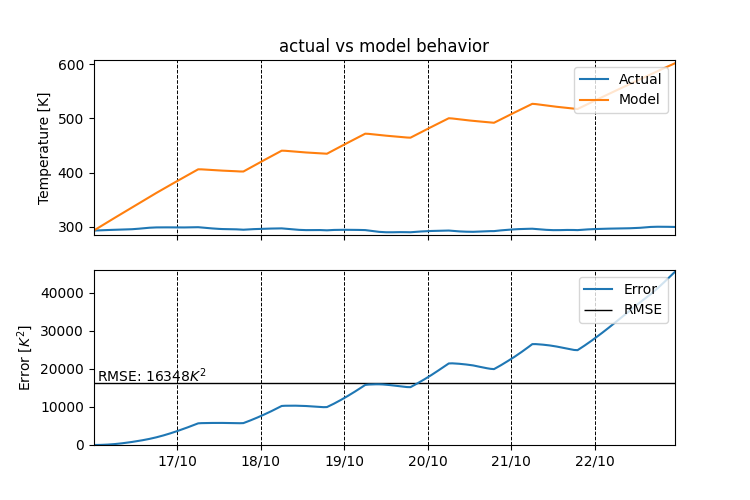
\includegraphics[scale=0.75]{images/error_actualvsmodel.png}
\caption{Predicted temperature model $\tilde{T}_{z}$ vs Actual temperature $T_z$ }
\label{fig:Model Error}
\end{figure}

\begin{python}
def minimize_function(Tz_a):
    N = len(Tz_a)
    delta_t = 3600  # s

    data = read_csv("leuven_october2022_16-22.csv")

    # Time dependent parameters
    time = data['time'].tolist()
    temp = data['temp'].tolist()  # deg C
    for i in range(len(temp)):
        temp[i] = temp[i] + 273.15  # deg K

    Qg = np.zeros(len(time))
    Qh = np.zeros(len(time))
    for i in range(5):
        Qg[0 + 24 * (i + 1):7 + 24 * (i + 1)] = 100  # W. Human heat 
        Qg[18 + 24 * (i + 1):24 + 24 * (i + 1)] = 100 

        Qh[0 + 24 * (i + 1):6 + 24 * (i + 1)] = 1000  # W. Heater
        Qh[19 + 24 * (i + 1):24 + 24 * (i + 1)] = 1000

    Qg[0:24] = 100
    Qg[144:] = 100
    Qh[0:24] = 1000
    Qh[144:] = 1000

    Qsun = data['solrad'].tolist()  # W/m2

    # Initiating optimization variables
    opti = Opti()
    R = opti.variable()
    C = opti.variable()
    gA = opti.variable()

    p = vertcat(R, C, gA)  # parameter vector

    Tz = 293.15  # Initial temperature guess

    f = 0   # Error function initial value

    for i in range(N):
        f = f + (Tz - Tz_a[i]) ** 2
        Tz_next = delta_t * ((Qsun[i] * gA + Qh[i] + Qg[i]) / C + (temp[i] - Tz) / (R * C)) + Tz
        Tz = Tz_next
        
    f = f + (Tz - Tz_a[N - 1]) ** 2

    opti.minimize(f)

    opti.solver('ipopt')

    # filling initial guess parameter vector
    p_hat = vertcat(R_guess, C_guess, gA_guess)

    opti.set_initial(p, p_hat)

    sol = opti.solve()

    return sol.value(p)
\end{python}


